% !TeX root = Bericht_main.tex

\subsection{Aufgabe 27}
In dieser Aufgabe betrachten wir die Konvektions-Diffusions-Reaktions-Gleichung
\begin{align*}
  \partial_t c = \dive (\kappa_c \nabla c - cq) + r(c)
\end{align*}
im Gebiet $Mesh=Square500$. Dabei wird zum Zeitpunkt
$t=0$ eine Bakterienkolonie mit der Konzentration $c_0(x)$ platziert. Der Reaktionsterm $r(c)$ ist durch
\begin{align*}
  r(c) = Rc
\end{align*}
gegeben.
\subsubsection{Aufgabe 27.1}

\begin{figure}[H]
	\centering
	\captionabove{Verlauf der Masse und des Ausflusses
	(Konvektion = 1)}
	\subfigure[Reaction = -2.5]{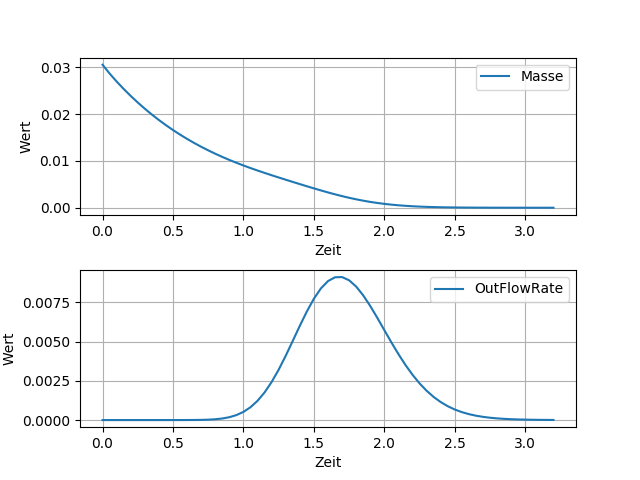
\includegraphics[width=0.32\textwidth]{../Aufgabe27/a/reaction=-2.5/plot.png}}
	\subfigure[Reaction = -1]{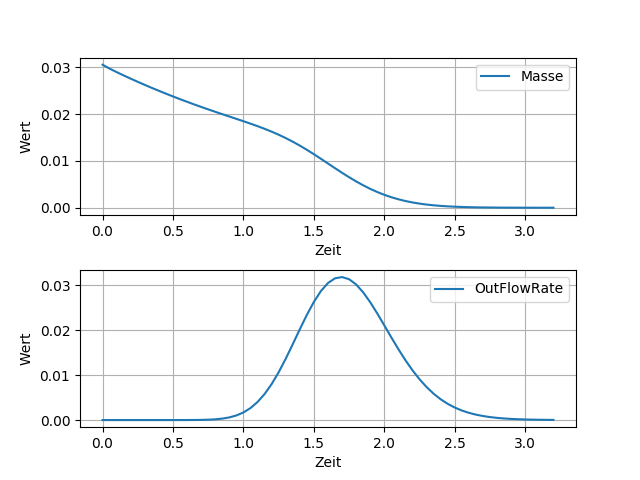
\includegraphics[width=0.32\textwidth]{../Aufgabe27/a/reaction=-1/plot.png}}
	\subfigure[Reaction = 0]{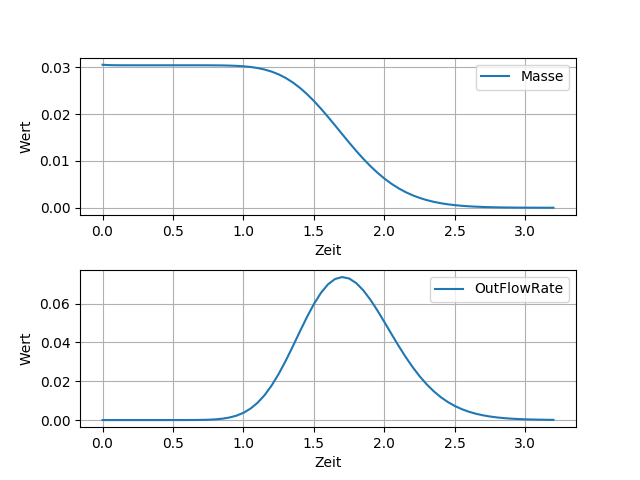
\includegraphics[width=0.32\textwidth]{../Aufgabe27/a/reaction=0/plot.png}}
	\subfigure[Reaction = 1]{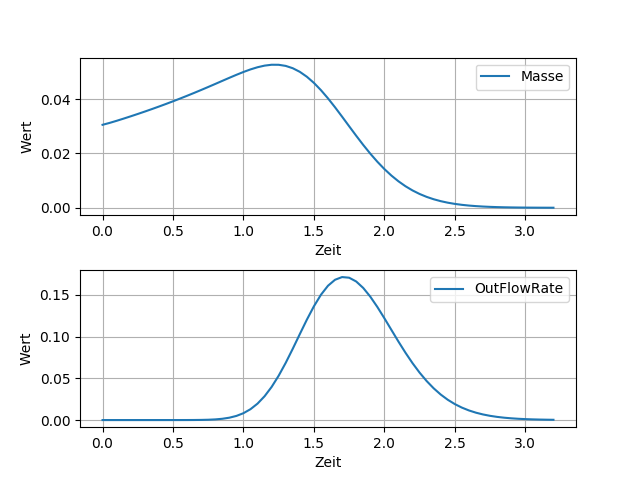
\includegraphics[width=0.32\textwidth]{../Aufgabe27/a/reaction=1/plot.png}}
	\subfigure[Reaction = 2.5]{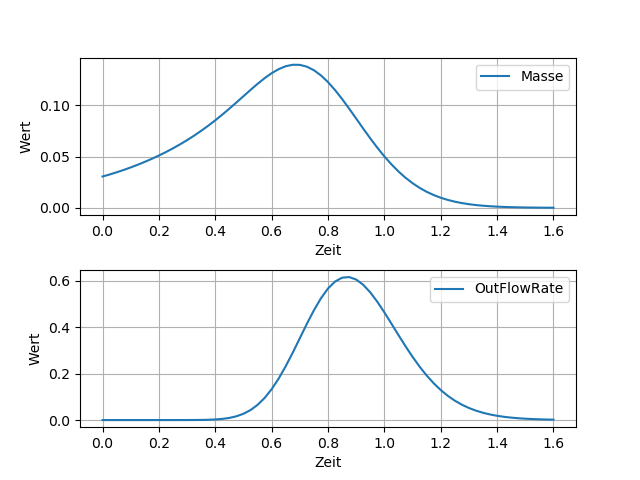
\includegraphics[width=0.32\textwidth]{../Aufgabe27/a/reaction=2.5/plot.png}}
	\subfigure[Reaction = 5]{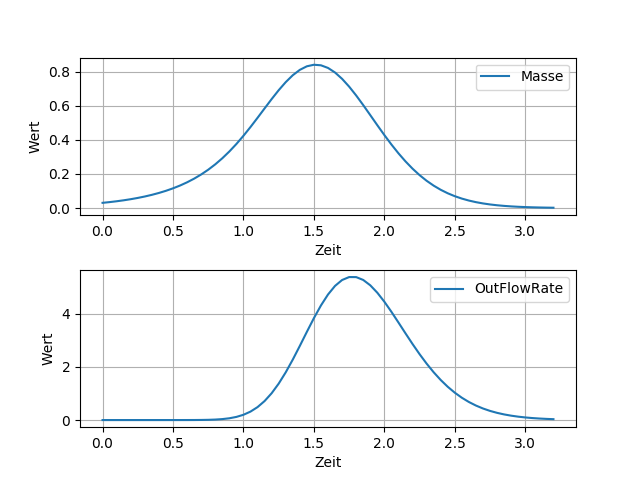
\includegraphics[width=0.32\textwidth]{../Aufgabe27/a/reaction=5/plot.png}}
\end{figure}

Anhand der Bilder erkennt man bei den negativen Reaktionsraten
den exponentiellen Zerfall der Masse, bei den positiven Reaktionsraten das exponentielle Wachstum der Masse bis zum Zeitpunkt $T=0.6$ sehr schön. Ab diesem Zeitpunkt überwiegt der Ausfluss des Fluids so stark, dass man den exponentiellen Verlauf ab nicht mehr beobachten kann.
Wird die Reaktion auf $0$ gesetzt erkennt man auch gut, dass sich die Konzentration der Bakterienkolonie nicht verändert und somit auch die Masse innerhalb des Gebietes bis zum Beginn des Ausflusses konstant bleibt.
Insgesamt bleibt außerdem festzuhalten, dass der Ausfluss nicht von der Reaktionsrate abhängt. 
Im Folgenden betrachten wir das Problem nochmals für eine niedrigere Konvektion:

\begin{figure}[H]
	\centering
	\captionabove{Verlauf der Masse und des Ausflusses (Konvektion = 0.1)}
	\subfigure[Reaction = 2.5]{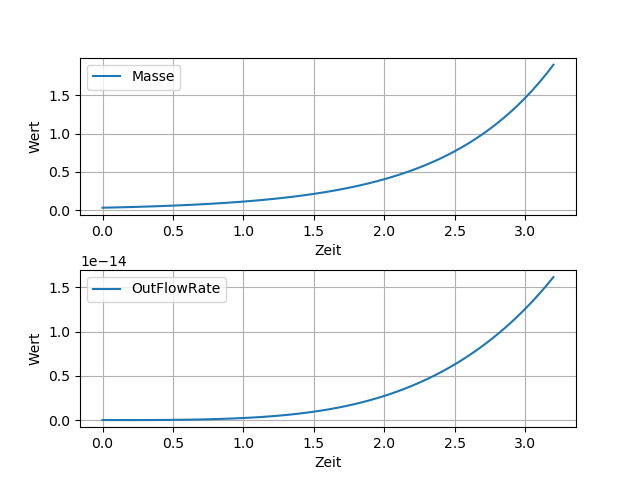
\includegraphics[width=0.99\textwidth]{../Aufgabe27/lowconvecreaction=2.5/plot.png}}
\end{figure}

\begin{figure}[H]
	\centering
	\captionabove{Verlauf der Masse und des Ausflusses (Konvektion = 0.1)}
	\subfigure[Reaction = 2.5]{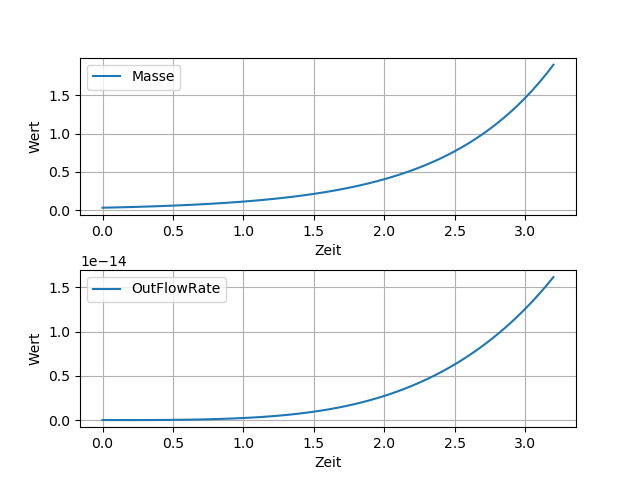
\includegraphics[width=0.32\textwidth]{../Aufgabe27/lowconvecreaction=2.5/plot.png}}
	\subfigure[Reaction = 2.5]{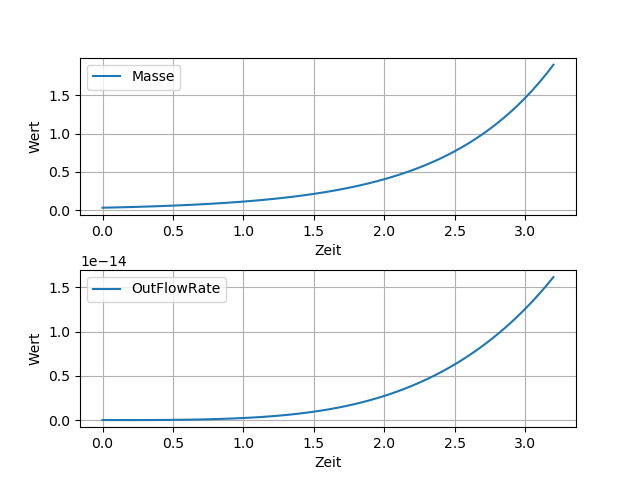
\includegraphics[width=0.32\textwidth]{../Aufgabe27/lowconvecreaction=2.5/plot.png}}
	\subfigure[Reaction = 2.5]{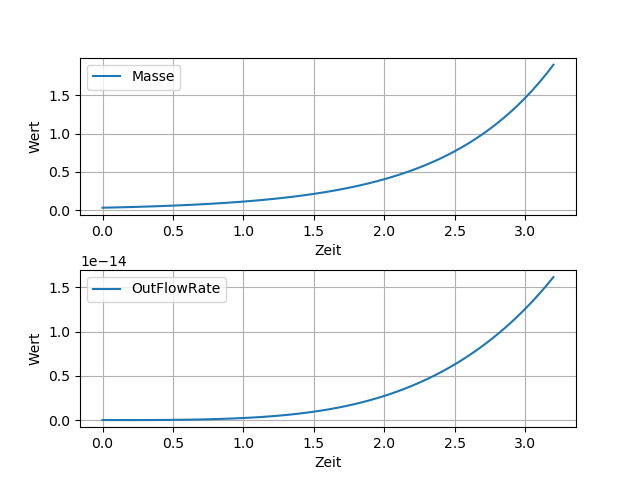
\includegraphics[width=0.32\textwidth]{../Aufgabe27/lowconvecreaction=2.5/plot.png}}
\end{figure}
\subsubsection{Aufgabe 27.2}
